
%(BEGIN_QUESTION)
% Copyright 2011, Tony R. Kuphaldt, released under the Creative Commons Attribution License (v 1.0)
% This means you may do almost anything with this work of mine, so long as you give me proper credit

This heat exchanger's outlet temperature is controlled by a PID controller, regulating the amount of steam admitted to the exchanger to impart heat to the process fluid:

$$\includegraphics[width=15.5cm]{i00297x01.eps}$$

An operator tells you there is a problem with this system, though: the controller faceplate shows the temperature well above setpoint.  You happen to notice that the bargraph on the controller faceplate showing output is at 0\%.  Another operator in the field (near the exchanger) reports via radio that the control valve stem is at the ``closed'' position.

\vskip 10pt

Another instrument technician happens to be with you, and recommends the controller be placed in manual mode for a quick stroke-test of the control valve (i.e. making sure it responds to the controller's output).  Explain why this test would be a waste of time, and propose a better test for helping to pinpoint the location of the fault.

\vskip 20pt \vbox{\hrule \hbox{\strut \vrule{} {\bf Suggestions for Socratic discussion} \vrule} \hrule}

\begin{itemize}
\item{} A valuable principle to apply in a diagnostic scenario such as this is {\it correspondence}: identifying which field variables correspond with their respective controller faceplate displays, and which do not.  Apply this comparative test to the scenario described, and use it to explain why the technician's proposed test was probably not the best first step.
\end{itemize}

\underbar{file i00297}
%(END_QUESTION)





%(BEGIN_ANSWER)

The reason that the technician's proposed test would have been a waste of time is because the control valve is already doing what the controller is telling it to: go to the 0\% (closed) position.  In other words, the valve stem position corresponds with the controller's output indication, suggesting there is no problem in that (output) portion of the control system.
 
\vskip 10pt

The controller's ``decision'' to shut the valve makes no sense from the perspective of PV $>$ SP.  What the controller should be doing is opening the cold feed valve in order to reduce the temperature of the process.  We do not know if the PV indication corresponds with the temperature gauge, but this is actually a moot point right now because we know for certain that the controller is not taking the correct action for what it ``sees'' in terms of PV and SP.  Fault possibilities include:

\begin{itemize}
\item{} Controller left in manual mode (not automatic)
\item{} Very poor controller tuning
\item{} Incorrect controller action
\end{itemize}

A good ``next step'' would be to check to see if the controller is in automatic mode.  If it is, then there is a problem with the controller's configuration or tuning.

%(END_ANSWER)





%(BEGIN_NOTES)


%INDEX% Basics, control loop troubleshooting: isolating area of fault by correspondence

%(END_NOTES)


